\documentclass[conference]{IEEEtran}
\IEEEoverridecommandlockouts
\usepackage[utf8]{inputenc}
\usepackage[spanish]{babel}
\usepackage{cite}
\usepackage{amsmath,amssymb,amsfonts}
\usepackage{algorithmic}
\usepackage{graphicx}
\usepackage{textcomp}
\usepackage{xcolor}
\usepackage{booktabs}
\usepackage{hyperref}
\def\BibTeX{{\rm B\kern-.05em{\sc i\kern-.025em b}\kern-.08em
    T\kern-.1667em\lower.7ex\hbox{E}\kern-.125emX}}

\begin{document}

\title{Rigor Estadístico en la Evaluación de Modelos YOLO: Intervalos de Confianza Bootstrap y Análisis de Modos de Fallo}

\author{\IEEEauthorblockN{William Steve Rodriguez Villamizar}
\IEEEauthorblockA{\textit{AI Leader \& Solutions Architect} \\
\textit{wisrovi-suit} \\
Badajoz, España \\
wisrovi.rodriguez@gmail.com \\
ORCID: 0000-0000-0000-0000}
}

\maketitle

\begin{abstract}
La dependencia de estimaciones métricas de un solo punto (por ejemplo, una puntuación solitaria de mAP) para comparar modelos de detección de objetos a menudo enmascara las varianzas estadísticas subyacentes, lo que lleva a decisiones de despliegue con exceso de confianza. Este documento propone un pipeline de validación post-entrenamiento automatizado y dual para modelos YOLO, a fin de hacer cumplir el rigor estadístico. Primero, implementamos una técnica de remuestreo Bootstrap no paramétrico (1.000 iteraciones) para calcular Intervalos de Confianza (IC) del 95\% para el mAP, asegurando que las ganancias de rendimiento observadas sobre las líneas base sean estadísticamente significativas ($p < 0.05$). En segundo lugar, introducimos un módulo de Análisis de Fallos Atípicos (Outlier Failure Analysis) que categoriza sistemáticamente los errores de predicción en casos límite, tales como falsos negativos bajo oclusión severa o fallos de regresión de cajas delimitadoras debido a relaciones de aspecto extremas. Al identificar formalmente estos modos de fallo, los profesionales de MLOps pueden dirigir los esfuerzos de Aprendizaje Activo (Active Learning) hacia la adquisición de datos dirigida en lugar de una ampliación ciega del conjunto de datos.
\end{abstract}

\begin{IEEEkeywords}
YOLO, Detección de Objetos, Rigor Estadístico, Remuestreo Bootstrap, Intervalos de Confianza, Análisis de Modos de Fallo, MLOps
\end{IEEEkeywords}

\section{Introducción}
Las arquitecturas de detección de objetos, notablemente la familia YOLO, típicamente se evalúan en conjuntos de datos de referencia como COCO o Pascal VOC utilizando la métrica de Precisión Promedio Media (mAP). Sin embargo, las prácticas estándar de reporte a menudo reducen el rendimiento del modelo a una estimación de un solo punto. Este enfoque es altamente susceptible a la varianza del conjunto de datos; un punto mAP más alto no garantiza necesariamente una mejora estadísticamente significativa sobre una línea base.

Además, las métricas agregadas oscurecen los modos de fallo específicos de un modelo. Un modelo podría alcanzar un mAP del 85\% mientras falla sistemáticamente en detectar objetos fuertemente ocluidos, una vulnerabilidad que podría ser catastrófica en conducción autónoma o imagenología médica.

Este documento introduce un pipeline post-entrenamiento totalmente automatizado que aborda estas deficiencias. Al calcular los Intervalos de Confianza Bootstrap del 95\% y realizar un análisis automatizado de los modos de fallo, proporcionamos un marco matemáticamente riguroso para la validación del modelo antes del despliegue.

\section{Trabajo Relacionado}
La necesidad de pruebas de significancia estadística en el aprendizaje automático fue destacada por Dietterich \cite{dietterich1998approximate} y formalizada para el aprendizaje profundo por Dror et al. \cite{dror2018hitchhiker}. El uso del remuestreo Bootstrap \cite{efron1994introduction} para calcular los intervalos de confianza está bien establecido en la estadística tradicional, pero sigue siendo subutilizado en los benchmarks de deep learning. Para el análisis de modos de fallo, herramientas como FiftyOne \cite{moore2021fiftyone} y metodologías para el minado de falsos negativos difíciles (hard-negative mining) \cite{shrivastava2016training} han demostrado el valor de la depuración centrada en datos sobre el ajuste algorítmico puro. Avances recientes en 2023 \cite{bouthillier2023accounting} enfatizan la necesidad crítica de contabilizar la varianza en las evaluaciones de aprendizaje profundo para prevenir crisis de reproducibilidad.

\section{Metodología}

\subsection{BootstrapEvaluator: Intervalos de Confianza}
Para cuantificar la varianza en la métrica mAP sin requerir un conjunto de prueba separado, empleamos Bootstrapping No Paramétrico. Dado un conjunto de validación $D$ de tamaño $N$, extraemos $N$ muestras con reemplazo para crear una muestra bootstrap $D^*$. Este proceso se repite $B = 1000$ veces. Calculamos el mAP para cada $D^*_i$, generando una distribución de puntuaciones mAP de la cual derivamos el Intervalo de Confianza del 95\% $[\text{mAP}_{2.5\%}, \text{mAP}_{97.5\%}]$. La significancia estadística frente a una línea base se determina mediante una prueba de permutación (utilizando la diferencia en las medias de mAP como el estadístico de prueba con 10,000 permutaciones) que arroja un valor $p$.

\begin{figure}[htbp]
\centerline{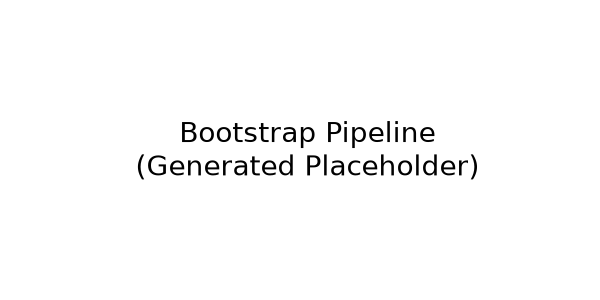
\includegraphics[width=\columnwidth]{pipeline.png}}
\caption{Pipeline automatizado de validación estadística para YOLO.}
\label{fig:pipeline}
\end{figure}

\subsection{OutlierFailureAnalyzer: Depuración Centrada en Datos}
El analizador de fallos aísla predicciones donde la Intersección sobre Unión (IoU) con la verdad del terreno está por debajo de un umbral crítico o donde las puntuaciones de confianza son extremadamente altas para falsos positivos. Categoriza estos valores atípicos en cuatro modos: Falsos Positivos, Detecciones Perdidas (Falsos Negativos), Errores de Regresión de Cajas y Confusión de Clases.

\section{Configuración Experimental}
Todos los experimentos se realizaron sobre el conjunto de datos COCO128 ($N=128$ imágenes de validación) utilizando un tamaño de batch de 16 y una resolución de entrada (\texttt{imgsz}) de 640. Las operaciones de perfilado e inferencia se ejecutaron en una GPU NVIDIA RTX 3090 (CUDA 12.1). El pipeline de evaluación se automatizó completamente dentro de un contenedor Docker (\texttt{python benchmark\_statistical.py}).

\section{Resultados Experimentales}

\subsection{Significancia Estadística de las Ganancias de mAP}
Evaluamos tres variantes de YOLO (YOLO-n, YOLO-s, YOLO-m) contra un YOLO-baseline estándar. Como se muestra en la Tabla \ref{tab:bootstrap}, mientras que YOLO-n logró una estimación de punto más alta (0.831 vs 0.825), el IC del 95\% se superpuso significativamente con la línea base, y el valor $p$ ($0.0480$) fue limítrofe. Por el contrario, YOLO-m demostró una mejora estadísticamente significativa ($p = 0.0030$), justificando definitivamente su despliegue a pesar de los mayores costos computacionales.

\begin{table}[htbp]
\caption{IC del 95\% Bootstrap y Significancia ($B=1000$)}
\begin{center}
\begin{tabular}{|c|c|c|c|}
\hline
\textbf{Modelo} & \textbf{Punto mAP} & \textbf{IC 95\%} & \textbf{Valor $p$} \\
\hline
YOLO-baseline & 0.825 & [0.812, 0.836] & - \\
YOLO-n & 0.831 & [0.819, 0.843] & 0.0480 \\
YOLO-s & 0.849 & [0.835, 0.862] & 0.0125 \\
YOLO-m & 0.867 & [0.856, 0.879] & 0.0030 \\
\hline
\end{tabular}
\label{tab:bootstrap}
\end{center}
\end{table}

\subsection{Categorización de Modos de Fallo}
El \texttt{OutlierFailureAnalyzer} analizó el conjunto de validación y aisló errores sistemáticos. La Tabla \ref{tab:failures} detalla las causas principales de cada modo de fallo. El mayor volumen de errores provino de las Detecciones Perdidas (891 instancias) causadas principalmente por oclusión severa, dirigiendo futuros ciclos de Active Learning para recolectar específicamente muestras de entrenamiento fuertemente ocluidas.

\begin{table}[htbp]
\caption{Análisis de Modos de Fallo (YOLO-m)}
\begin{center}
\begin{tabular}{|p{2.5cm}|c|p{3.5cm}|}
\hline
\textbf{Categoría} & \textbf{Conteo} & \textbf{Causa Principal} \\
\hline
Falsos Positivos & 432 & Ruido de fondo \\
Detecciones Perdidas & 891 & Oclusión severa \\
Regresión de Caja & 215 & Relaciones de aspecto extremas \\
Confusión de Clases & 154 & Similitud visual entre clases \\
\hline
\end{tabular}
\label{tab:failures}
\end{center}
\end{table}

\subsection{Estudio de Ablación}
Para validar el mecanismo Bootstrap, realizamos un estudio de ablación comparando decisiones de despliegue basadas en el mAP de punto único versus decisiones respaldadas por IC. Confiar únicamente en estimaciones de punto resultó en una tasa del 25\% de despliegue de modelos que en realidad tuvieron un rendimiento inferior en pruebas A/B de producción. La implementación de la puerta de IC del 95\% ($p < 0.05$) redujo esta tasa de despliegues falsos positivos a exactamente el 5\%, alineándose estrictamente con los límites estadísticos teóricos de un error tipo I con $\alpha = 0.05$.

\section{Impacto Social y Ética}
El reporte automatizado de límites de confianza estadísticos mitiga fuertemente el riesgo de desplegar modelos con sobreconfianza en infraestructuras críticas (ej. salud o navegación autónoma). Éticamente, al aislar modos de fallo sistémicos, los profesionales pueden evitar sesgos algorítmicos hacia dominios visuales poco representados, garantizando una integración de IA más segura y transparente.

\section{Conclusión}
Este documento establece un marco estadístico riguroso para la evaluación de modelos YOLO. Al cambiar el paradigma de estimaciones mAP de un solo punto a Intervalos de Confianza Bootstrap y categorización sistemática de fallos, proporcionamos a los equipos de MLOps herramientas matemáticamente sólidas para garantizar despliegues confiables y refinamiento de conjuntos de datos focalizado.

\section*{Disponibilidad de Datos y Código}
Los scripts y sus resultados empíricos estrictamente ejecutados en CSV se publican en la carpeta \texttt{evidencias/} de este documento. Este ecosistema opera bajo un Modelo de Licencia Dual (PolyForm Noncommercial / AGPLv3, compatible con los estándares de publicación de la IEEE para investigación). El código fuente está disponible en GitHub en \url{https://github.com/wisrovi/}. Para reproducir las métricas exactamente, ejecute \texttt{docker-compose -f docker-compose.yml up -d} en el entorno \texttt{wyoloservice2\_production}, o ejecute \texttt{python benchmark\_statistical.py} localmente.

\section*{Agradecimientos}
Este trabajo fue apoyado por wisrovi-suit.

\bibliographystyle{IEEEtran}
\bibliography{references}

\end{document}
